\chapter{Lesson 4}
\section{Overview}
In lesson one of this special feature on learning the guitar, we were introduced to the parts of the guitar, learned to tune the instrument, learned a chromatic scale, and learned Gmajor, Cmajor, and Dmajor chords. Guitar lesson two taught us to play Eminor, Aminor, and Dminor chords, an E phrygian scale, a few basic strumming patterns, and the names of the open strings. In guitar lesson three, we learned how to play a blues scale, Emajor, Amajor, and Fmajor chords, and a new strumming pattern. If you are not familiar with any of these concepts, it is advised that you revisit these lessons before proceeding.

\subsection{What You'll Learn in Guitar Lesson Four}

We'll start adventuring a little farther up the neck in this lesson. You'll learn a new type of chord... what is known as a "power chord". You'll also learn the names of the notes on the sixth and fifth string. Plus, of course, strumming patterns, and a bunch more songs to play. Let's start guitar lesson four.

\section{The Musical Alphabet on Guitar}
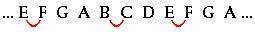
\includegraphics{partfour/musalph.jpg}

So far, most of what we've learned on the guitar has been focused on the bottom few frets of the instrument. Most guitars have at least 19 frets - by only using the first three, we aren't using the instrument as effectively as we could. Learning the notes all over the guitar fretboard is the first step we need to take to unlock the instrument's full potential

\subsection{The Musical Alphabet}

Before we begin, it is very important to understand the way the "musical alphabet" works. It is similar in many respects to the traditional alphabet, in that it uses standard letters (remember your ABCs?). In the musical alphabet, however, the letters only progress up to G, after which they begin again at A. As you continue up the musical alphabet, the pitches of the notes get higher (when you go past G up to A again, the notes continue to get higher, they don't start at a low pitch again.)

Another complication of learning the musical alphabet on guitar is that there are extra frets in between some, but not all of these note names. The graphic above is an illustration of the musical alphabet. The ties between the notes B and C, and also between the notes E and F, reflect the fact there is NO "blank" fret between these two sets of notes. Between ALL OTHER notes, there is one fret space.

This rule applies to all instruments, including piano. If you are familiar with the piano keyboard, you will know that there is no black key between the notes B and C, and also E and F. But, between all other sets of notes, there is a black key.

SUMMARY: On the guitar, there are no frets between the notes B\&C, and between E\&F. Between all other notes, there is one (for now, unnamed) fret between each.

\section{Notes on the Neck}
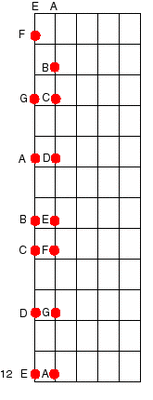
\includegraphics{partfour/fretboard.png}

From guitar lesson two, you'll remember that the name of the open sixth string is "E". Now, let's figure out the other note names on the sixth string.

Coming after E in the musical alphabet is... you guessed it... F. Referencing the musical alphabet we just learned, we know there is no blank fret between these two notes. So, F is on the sixth string, first fret. Next, let's figure out where the note G is located. We know that there is a blank fret between F and G. So, count up two frets, and G is on the third fret of the sixth string. After G, in the musical alphabet, comes the note A again. Since there is a blank fret between G and A, we know that A is on the fifth fret of the sixth string. Continue this process all the way up the sixth string. You can check the diagram here to make sure you are correct.

Remember: there is also no blank fret between the notes B and C.

Once you reach the 12th fret (which is often marked on the neck of the guitar by double dots), you'll notice you have reached the note E again. You'll find on all six strings that the note on the 12th fret is the same as the open string.

Once you've finished counting up the E string, you'll want to try the same exercise on the A string. This shouldn't be difficult... the process is exactly the same as it was on the sixth string. All you need to know is the name of the open string to get started.

Unfortunately, understanding how to figure out note names on the fretboard isn't enough. For these note names to be useful, you'll have to go about memorizing them. The best way to memorize the fretboard is to commit several note names and frets to memory on each string. If you know where A is on the sixth string, for example, it will be much easier to find the note B. For now, we'll just worry about memorizing the notes the sixth and fifth strings.

In lesson five, we will fill in the blank frets in the diagram with note names. These names include sharps (?) and flats (?). Before you start learning these other notes, however, you'll need to understand and memorize the above notes.

\subsection{THINGS TO REMEMBER:}
\begin{itemize}
\item The musical alphabet goes from A to G, then back to A again.
\item There is no blank fret between the notes B\&C, and E\&F.
\item The note name on the 12th fret of any string is always the same as the open string.
\item Memorize the open string name, and several more note names and locations on both the sixth and fifth string. This will make finding all other notes much quicker.
\end{itemize}

\section{Power Chords}
In order to learn power chords effectively, you'll need to really understand the names of the notes on the neck of the guitar. If you glossed over that page, you'll want to revisit it, and learn it well.

\subsection{What a Power Chord Is}

In some styles of music, particularly in rock and roll, it's not always necessary to play a big, full sounding chord. Often, especially on an electric guitar, it sounds best to play two-or-three note chords. This is when power chords come in handy.

Power chords have been popular since the birth of blues music, but when grunge music started to rise in popularity, many bands chose to use power chords almost exclusively, instead of more "traditional" chords. The power chords we are about to learn are "movable chords", meaning that, unlike the chords we've learned so far, we can move their position up or down the neck, to create different power chords.

Although the power chord pictured here contains three notes, the chord contains only two *different notes* - one note is doubled an octave higher. A power chord contains the "root note" - the root of a C power chord is "C" - and another note called the "fifth". For this reason, power chords are often referred to as "fifth chords" (written C5 or E5, etc).

The power chord does not contain the note which traditionally tells us whether a chord is major or minor. Thus, a power chord is neither major nor minor. It can be used in a situation where either a major or a minor chord is called for, however. Take a look at this example of a chord progression:

Cmajor - Aminor - Dminor - Gmajor

We could play the above progression with power chords, and we'd play it as follows:

C5 - A5 - D5 - G5

\subsection{Power chords on the sixth string}
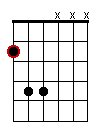
\includegraphics{partfour/powerchord6.png}

Take a look at the diagram above - note that you do NOT play the third, second, and first strings. This is important - if any of these strings ring, the chord won't sound very good. You'll also notice that the note on the sixth string is circled in red. This is to denote that the note on the sixth string is the root of the chord. This means that, while playing the power chord, whatever note is being held down on the sixth string is the name of the power chord.

For example, if the power chord were being played starting on the fifth fret of the sixth string, it would be referred to as an "A power chord", since the note on the fifth fret of the sixth string is A. If the chord were played on the eighth fret, it would be a "C power chord". This is why it is important to know the names of the notes on the sixth string of the guitar.

Play the chord by placing your first finger on the sixth string of the guitar. Your third (ring) finger should be placed on the fifth string, two frets up from your first finger. Lastly, your fourth (pinky) finger goes on the fourth string, on the same fret as your third finger. Strum the three notes with your pick, making sure that all three notes ring clearly, and that all are of equal volume.

\subsection{Power chords on the fifth string}
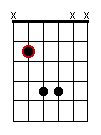
\includegraphics{partfour/powerchord5.png}

If you can play the power chord on the sixth string, this one should be no trouble at all. The shape is exactly the same, only this time, you'll need to be sure you don't play the sixth string. Many guitarists will overcome this problem by lightly touching the tip of their first finger against the sixth string, deadening it so it doesn't ring.

The root of this chord is on the fifth string, so you'll need to know what the notes are on this string in order to know what power chord you're playing. If, for example, you're playing a fifth string power chord on the fifth fret, you are playing a D power chord.

\subsection{Things to Know About Power Chords:}
\begin{itemize}
\item Power chords are often referred to as a "fifth" or "5" chord. If you see a chord written as C5, it is a C power chord
\item You can optionally omit the pinky finger, and play a power chord as a two-note chord. Most guitarists stick with the 3-note version, as they sound more full
\item A common fingering for a power chord is to play the root note with the first finger, while the third finger barres the other two notes
\item Power chords are generally used in pop, rock, and blues music. Because they are not big, full sounding chords, power chords are not commonly used in acoustic strumming situations
\item Many guitarists prefer to use all downstrokes when strumming power chords. This results in a more "chunky" sound. This is not a rule, only an observation
\end{itemize}

\section{F Major Chord Review}
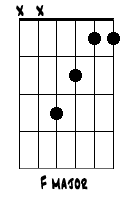
\includegraphics{partfour/chord_fmajor_open.png}

It might seem silly to devote an entire page to going over one chord we've already learned, but, believe me, you will appreciate it in coming weeks. The F major chord is the most difficult we've learned thus far, but it uses a technique that we will use constantly in future lessons. That technique is using one finger in your fretting hand to hold down more than one note at a time.

\subsection{The F major shape}

In case you're having trouble remembering how to play the chord, let's go over it again. Your third finger plays the third fret on the fourth string. Your second finger plays the second fret on the third string. And, your first finger plays the first fret on both the second and first strings. Make sure when you strum the chord that you're not playing the sixth and fifth strings.

Many guitarists find that slightly rolling the first finger back (towards the headstock of the guitar) makes playing the chord slightly easier. If, after you've done this, the chord still doesn't sound properly, play each string, one by one, and identify what the problem string(s) are. Keep practicing this chord - play it every day, and don't give up. It won't take long for the Fmajor chord to start sounding just as good as the rest of your chords do.

\subsection{Songs that use an F major chord}

There are, of course, thousands of songs that use an F major chord, but for practicing purposes, here are just a few. They may take some work to master, but you should have them sounding good with some solid practice. If have forgotten some of the other chords we've learned, you can check the guitar chord library.

Mother - performed by Pink Floyd
This is a good acoustic song to start with, because there aren't many chords, the changes are slow, and F major only occurs a couple of times.

Kiss Me - performed by Sixpence None the Richer
The strum for this song is tricky (we'll leave it alone for a while... for now, play quick downstrums 8x per chord, only 4x for the chorus). There are a few chords we might not have covered yet, but they should be explained at the bottom of the page. Not many F major chords... just enough to keep you challenged.

Night Moves - performed by Bob Seger
Just a quick F major in this song, so it might be a difficult tune to play at first. If you know the song well, this one will be much easier to play. 

\section{Strumming Patterns}
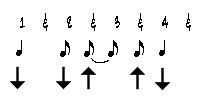
\includegraphics{partfour/strum4.png}

In lesson two, we learned all about the basics of strumming the guitar. We added another new strum to our repertoire in lesson three. If you still aren't comfortable with the concept and execution of basic guitar strumming, it is advised that you return to those lessons and review.

Just a slight variation from the strum we learned in lesson three gives us another very common, usable strumming pattern. In fact, many guitarists actually find this pattern to be slightly easier, as there is a slight pause at the end of the bar, which can be used to switch chords.

Before you try and play the strumming pattern above, take some time to learn what it sounds like. Listen to an mp3 clip of the strumming pattern, to and try to tap along with it. Repeat this until you can tap out this pattern without thinking about it.

Once you've learned the basic rhythm of this strum, pick up your guitar and try playing the pattern while holding down a Gmajor chord. Be sure to use the exact upstrokes and downstrokes the diagram illustrates - this will make your life much easier. If you're having trouble, put down the guitar and practice saying or tapping out the rhythm again. If you don't have the correct rhythm in your head, you'll never be able to play it on guitar. Once you're comfortable with the strum, try playing along with the same pattern at a faster tempo (listen to faster tempo strum here).

Again, remember to keep the up and down strumming motion in your picking hand constant - even when you're not actually strumming the chord. Try saying out loud "down, down up, up down" (or "1, 2 and, and 4") as you're playing the pattern.

\subsection{Things to Remember}
\begin{itemize}
\item If playing an acoustic guitar, make sure to strum directly over the sound hole
\item On electric guitar, strum over the body, not over the neck
\item Make sure all strings are ringing clearly
\item Make sure the volume of your downstrums and upstrums are equal
\item Don't strum too hard, as this causes strings to rattle, and produces an undesirable sound
\item Don't strum too softly, as this produces a "wimpy" sound. Your pick should be striking the strings with a relatively firm, even stroke
\item Think of your elbow as being the top of a pendulum; your arm should swing up and down from it in a steady motion, never pausing at any time.
\item Having said that, the bulk of the picking motion should come from a rotation of the wrist, rather than from the forearm. Be sure not to keep your wrist stiff when playing.
\end{itemize}

\section{Learning Songs}
Since we've now covered all the basic open chords, plus power chords, we have a lot of options in which songs we can play. This week's songs will be focus on both open and power chords.

Smells Like Teen Spirit (Nirvana)
This is perhaps the most famous of all grunge songs. It uses all power chords, so once you can play those comfortably, the song shouldn't be too hard.
MP3: "Smells Like Teen Spirit" at Amazon.com

Have You Ever Seen the Rain (CCR)
We can use our new strum with this fairly simple song. Although it does have a couple of chords we haven't covered yet, they should be explained well on the page.
MP3: "Have You Ever Seen the Rain" at Amazon.com

Still Haven't Found What I'm Looking For (U2)
Here's a nice, easy one to play, but unfortunately the tab is a little difficult to read. When trying to figure out this sheet music, be aware that the chord changes are UNDER the words, instead of over them, which is normally the case. MP3: "Still Haven't Found What I'm Looking For" at Amazon.com 

\section{Practice Schedule}
As we progress further in these lessons, it becomes more and more important to have daily practice time, as we're starting to cover some really tricky material. Power chords can take a while to get used to, so I suggest making a habit of playing them regularly. Here's a suggested use of your practice time for the next few weeks.
%
\begin{itemize}
\item Make sure your guitar is in tune (review how to tune).
\item Warm up by playing the chromatic scale, forwards and backwards, several times. Play slowly, use alternate picking, and make sure each note rings clearly.
\item Play the E phrygian scale from lesson two several times, paying careful attention to detail.
\item Review the names of notes on the sixth and fifth string. Practice calling out a random note (e.g. C), and trying to find that note on BOTH the sixth and fifth string. Memorize at least two other notes, and their positions on each string.
\item Work on your power chords. Make sure your ring finger is positioned well on the appropriate fret (it is the finger that most often makes power chords sound bad). Slide from chord to chord, and try moving from the 6th string power chords to the 5th string power chords.
\item Review all nine major and minor chords we've learned. You should really be close to memorizing all of these chords by now. Pick two chords, and practice moving from one to the next quickly and smoothly. Then, pick two new chords, and repeat the process.
\item Spend some time working on this week's new strumming pattern. Also, be sure to revisit the patterns from lesson two and lesson three. Try switching from chord to chord while using these patterns.
\item Work on playing that pesky F major chord. Don't give up until it sounds perfect. Try playing some of the songs listed on that page.
\item Try to play all of the songs in lesson four. Each of these songs has been chosen to help you work on a particular aspect of your guitar playing.
\end{itemize}
%
We are starting to build up a large archive of things to practice, so if you find it impossible to find the time to practice all of the above in one sitting, try breaking up the material, and practicing it over several days. There is a strong human tendency to only practice things which we are already quite good at. You'll need to overcome this, and force yourself to practice the things you are weakest at doing.

I can't emphasize strongly enough that it is important to practice everything we've done in these four lessons. Some things will undoubtedly be more fun than others, but trust me, the things you hate doing today are probably techniques that will become the basis for other things you will love to play in the future. The key to practice is, of course, fun. The more you enjoy playing guitar, the more you'll play, and the better you will get. Try to have fun with whatever you're playing.

In lesson five, we'll learn a blues shuffle, names of sharps and flats, a barre chord, plus more songs! Hang in there, and have fun!

